\documentclass[border=10pt]{standalone}
\usepackage[svgnames]{xcolor}
\usepackage{amsmath}
\usepackage{pgfplots}
\pgfplotsset{compat=newest}
\usepackage[sfdefault]{FiraSans}
\usepackage{FiraMono}
\renewcommand*\familydefault{\sfdefault}
\begin{document}
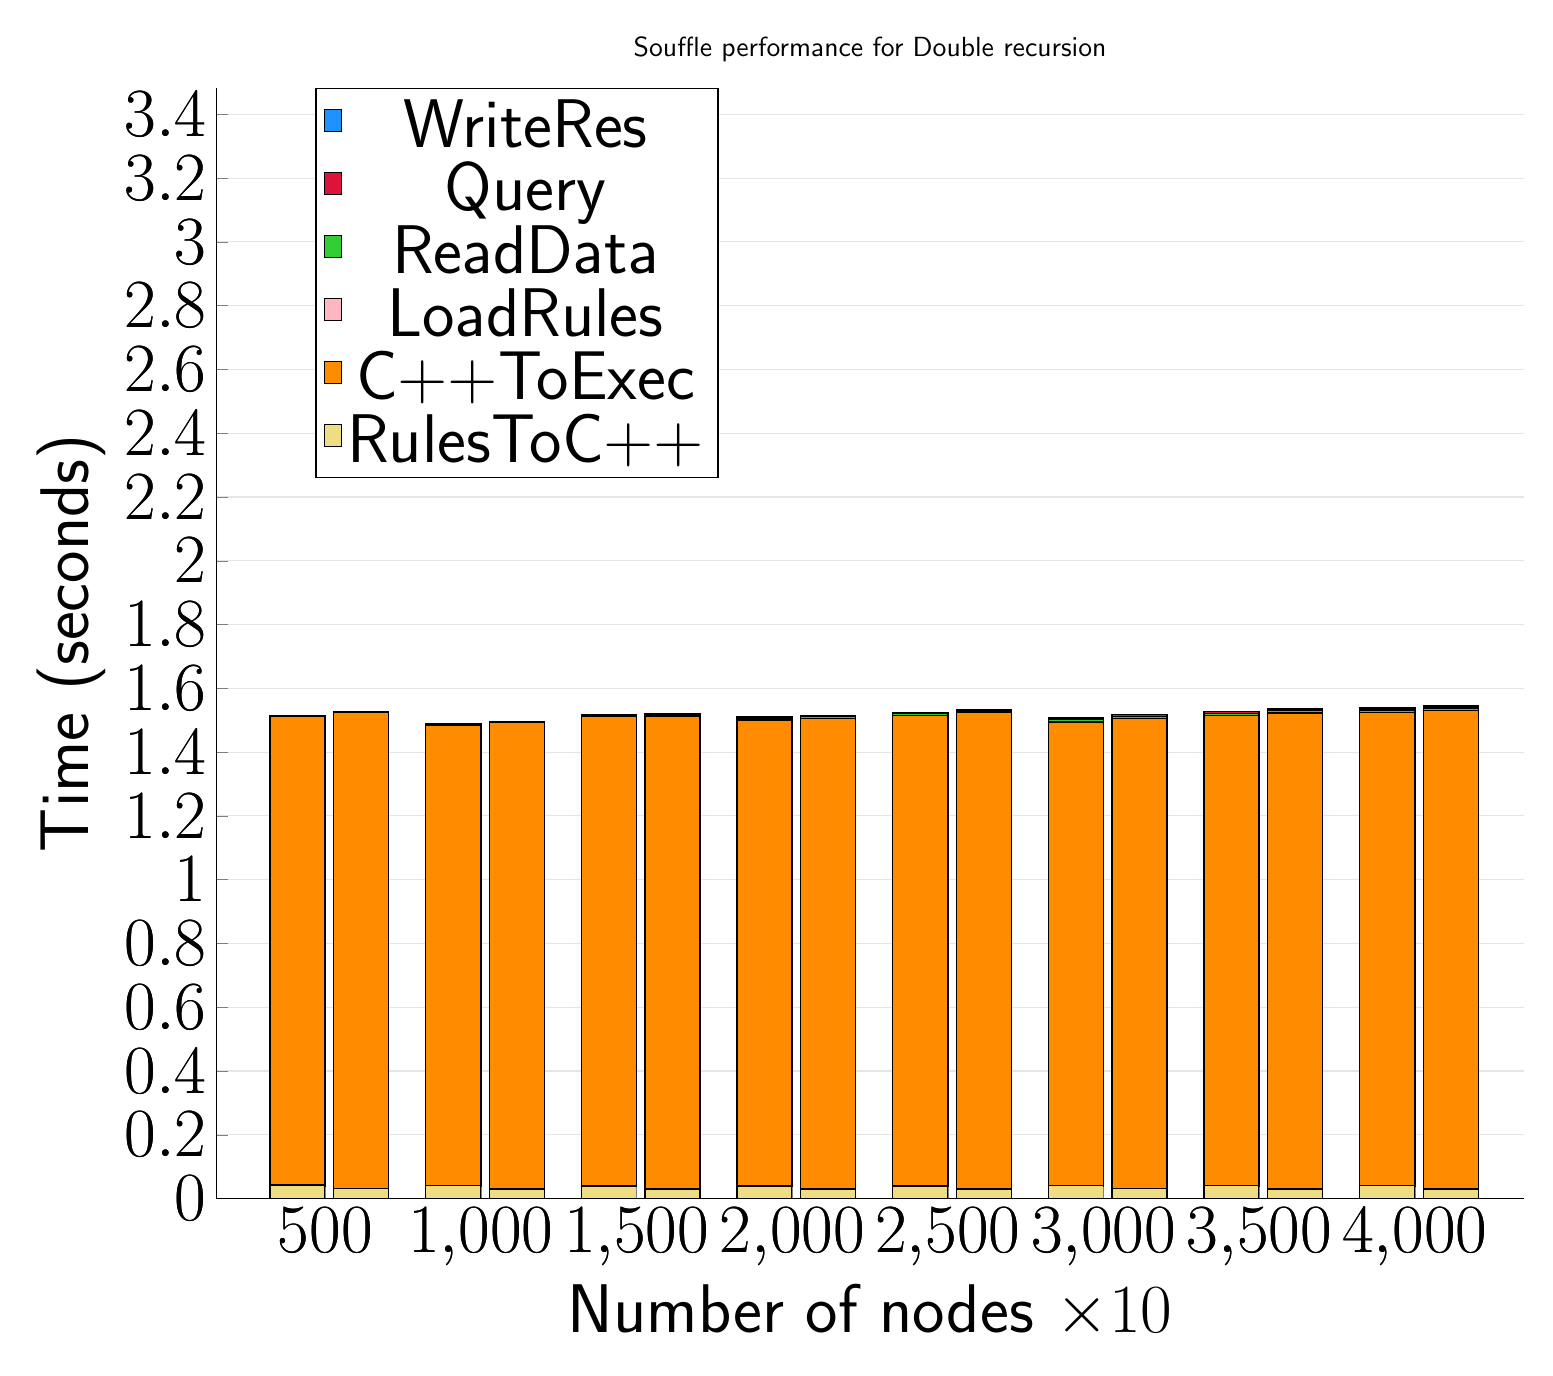
\begin{tikzpicture}
\begin{axis}[
   ybar stacked,
   title={Souffle performance for Double recursion},
   bar shift=-10pt,
   width=1.5\textwidth,
   bar width=0.7cm,
   ymajorgrids, tick align=inside,
   major grid style={draw=gray!20},
   xtick=data,
   ymin=0, ymax=3.4829999923706056,
   axis x line*=bottom,
   axis y line*=left,
   enlarge x limits=0.1,
   legend style={
       at={(0.23, 1)},
       anchor=north,
       legend columns=1,
       font=\Huge,
   },
   ylabel={Time (seconds)},
   xlabel={Number of nodes $\times 10$},
   label style={font=\Huge},
   tick label style={font=\Huge},
]
\addlegendimage{fill=DodgerBlue, draw=black, line width=0.2pt}
\addlegendentry{WriteRes}
\addlegendimage{fill=Crimson, draw=black, line width=0.2pt}
\addlegendentry{Query}
\addlegendimage{fill=LimeGreen, draw=black, line width=0.2pt}
\addlegendentry{ReadData}
\addlegendimage{fill=LightPink, draw=black, line width=0.2pt}
\addlegendentry{LoadRules}
\addlegendimage{fill=DarkOrange, draw=black, line width=0.2pt}
\addlegendentry{C++ToExec}
\addlegendimage{fill=LightGoldenrod, draw=black, line width=0.2pt}
\addlegendentry{RulesToC++}
\addplot +[fill=LightGoldenrod, draw=black, line width=0.5pt] coordinates {
    (500, 0.043000006675720216)
    (1000, 0.040999984741210936)
    (1500, 0.03900001049041748)
    (2000, 0.04000000953674317)
    (2500, 0.039999985694885255)
    (3000, 0.04100000858306885)
    (3500, 0.04100000858306885)
    (4000, 0.04100000858306885)
};
\addplot +[fill=DarkOrange, draw=black, line width=0.5pt] coordinates {
    (500, 1.4700000286102295)
    (1000, 1.4440000295639037)
    (1500, 1.472000002861023)
    (2000, 1.4609999656677246)
    (2500, 1.475000023841858)
    (3000, 1.4540000200271606)
    (3500, 1.4729999780654908)
    (4000, 1.4829999923706054)
};
\addplot +[fill=LightPink, draw=black, line width=0.5pt] coordinates {
    (500, 8.54749e-05)
    (1000, 0.00011490420000000001)
    (1500, 0.00012440839999999998)
    (2000, 0.00011062089999999999)
    (2500, 8.322920000000001e-05)
    (3000, 0.00010725419999999999)
    (3500, 8.075000000000001e-05)
    (4000, 0.00010856679999999999)
};
\addplot +[fill=LimeGreen, draw=black, line width=0.5pt] coordinates {
    (500, 0.0011643741000000002)
    (1000, 0.002502818)
    (1500, 0.0035307579999999997)
    (2000, 0.004697346000000001)
    (2500, 0.005101878999999999)
    (3000, 0.006559251)
    (3500, 0.007258903999999999)
    (4000, 0.008192658)
};
\addplot +[fill=Crimson, draw=black, line width=0.5pt] coordinates {
    (500, 0.0006586125999999999)
    (1000, 0.0015759840000000001)
    (1500, 0.00226033)
    (2000, 0.003017721)
    (2500, 0.0035758490000000003)
    (3000, 0.0044753910000000004)
    (3500, 0.005078738)
    (4000, 0.005698383)
};
\addplot +[fill=DodgerBlue, draw=black, line width=0.5pt] coordinates {
    (500, 0.00046044609999999997)
    (1000, 0.0007536827)
    (1500, 0.0008590791)
    (2000, 0.0010766272999999998)
    (2500, 0.0012540721000000002)
    (3000, 0.0016149330000000003)
    (3500, 0.0015138660000000002)
    (4000, 0.0018319210000000002)
};
\end{axis}
\begin{axis}[
   ybar stacked,
   bar shift=13pt,
   width=1.5\textwidth,
   bar width=0.7cm,
   ymajorgrids, tick align=inside,
   major grid style={draw=none},
   xtick=data,
   ymin=0, ymax=3.4829999923706056,
   axis x line*=none,
   axis y line*=none,
   enlarge x limits=0.1,
   label style={font=\Huge},
   tick label style={font=\Huge},
]
\addplot +[fill=LightGoldenrod, draw=black, line width=0.5pt] coordinates {
    (500, 0.031000000000000007)
    (1000, 0.030000000000000006)
    (1500, 0.030000000000000006)
    (2000, 0.030000000000000006)
    (2500, 0.030000000000000006)
    (3000, 0.030999999999999993)
    (3500, 0.030000000000000006)
    (4000, 0.030000000000000006)
};
\addplot +[fill=DarkOrange, draw=black, line width=0.5pt] coordinates {
    (500, 1.493)
    (1000, 1.4620000000000002)
    (1500, 1.483)
    (2000, 1.4760000000000002)
    (2500, 1.4940000000000002)
    (3000, 1.475)
    (3500, 1.493)
    (4000, 1.5)
};
\addplot +[fill=LightPink, draw=black, line width=0.5pt] coordinates {
    (500, 8.49e-05)
    (1000, 0.00011410000000000001)
    (1500, 0.0001239)
    (2000, 0.00010990000000000002)
    (2500, 8.26e-05)
    (3000, 9.669999999999999e-05)
    (3500, 8.04e-05)
    (4000, 0.00010779999999999999)
};
\addplot +[fill=LimeGreen, draw=black, line width=0.5pt] coordinates {
    (500, 0.0011630000000000002)
    (1000, 0.0025005)
    (1500, 0.0035295999999999995)
    (2000, 0.004693)
    (2500, 0.005098699999999999)
    (3000, 0.0065536)
    (3500, 0.0072546)
    (4000, 0.0081888)
};
\addplot +[fill=Crimson, draw=black, line width=0.5pt] coordinates {
    (500, 0.0006575000000000001)
    (1000, 0.0015742000000000002)
    (1500, 0.0022596999999999995)
    (2000, 0.003015)
    (2500, 0.0035719000000000007)
    (3000, 0.0044706)
    (3500, 0.0050712000000000005)
    (4000, 0.0056858)
};
\addplot +[fill=DodgerBlue, draw=black, line width=0.5pt] coordinates {
    (500, 0.00039709999999999995)
    (1000, 0.0006895)
    (1500, 0.0008583999999999999)
    (2000, 0.0010749000000000002)
    (2500, 0.001148)
    (3000, 0.0014338999999999999)
    (3500, 0.0015057999999999998)
    (4000, 0.0017131)
};
\end{axis}
\end{tikzpicture}

\end{document}
